\documentclass[12pt,titlepage]{article}
\usepackage[toc,page]{appendix}
\usepackage[linktoc=all]{hyperref}
\usepackage{listings}
\usepackage{graphicx}
\usepackage[margin=1in]{geometry}
\graphicspath{ {figures/} }
\usepackage{xcolor}
\usepackage{cite}
\usepackage{array}
\usepackage{titlesec}
\setcounter{secnumdepth}{6}
\title{Spiking Neural Network on an FPGA}
\author{ECE 07\\{\small{Cameron Calv, Neel Jagad, Nicholas Sica}}\\{\small{Advisor: Dr. Anup Das}}}
\date{February 26, 2021}
\linespread{1.25}
\begin{document}
\maketitle
\newpage
\clearpage
\pagenumbering{arabic}

\begin{abstract}
Sleep apnea is a potentially deadly affliction causing irregular or halted breathing during
	periods of sleep that many individuals will unknowingly suffer from in their lifetime. It 
	is usually diagnosed using polysomnography (PSG) testing either in a lab environment, which
	is costly and accurate, or in-home tests (IHT) where it is cheaper in exchange for underestimating
	the apnea’s severity. Machine learning has the potential to accurately predict sleep apnea severity
	using the same oxygen saturation levels as a PSG or IHT test. Deep learning has emerged as a vital
	subfield using a multi-layered architecture vaguely reminiscent of the human brain in its complexity,
	and it has shown to be incredibly accurate with the expense being increased power, complexity, and
	time requirements. The gap between PSG tests and IHTs may be reduced with a machine learning model
	that has the accuracy of the PSG tests and that can be implemented on the resource limited IHT kits.
	Bridging this gap will contribute to wider test availability while remaining economically feasible.
	Initially, spiking neural networks (SNN) have been observed to decrease power, computing, and time
	while being able to process in near real-time. Similarly, FPGAs (field-programmable gate arrays)
	have shown to further reduce power, computing, and time when such an SNN is programmed onto them. 
	In addition, the FPGA’s re-programmability makes it suitable to utilize any onboard SNN model. CPUs 
	and GPUs may be used to generate these models, while the FPGA will house them and make predictions 
	using the trained model’s rules. 
\end{abstract}

\tableofcontents

\listoffigures

\listoftables

\newpage

\section{Executive Summary}
\begin{table}[!htb]
	\label{tbl:quadchart}
	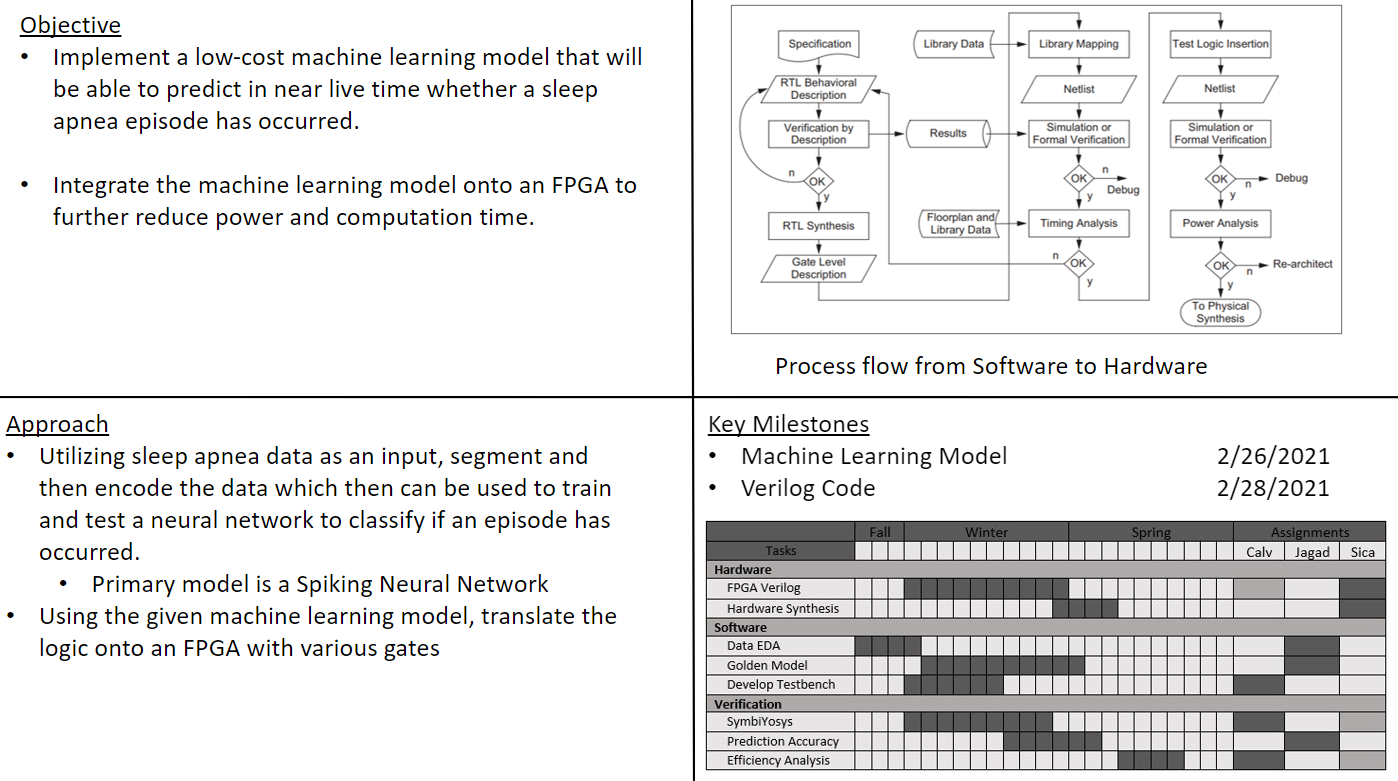
\includegraphics[width=\linewidth]{quadchart.png}
\end{table}

\section{Introduction}
\subsection{Motivation}
Sleep apnea is a sleeping condition which causes the airway to become blocked at various times throughout the night, which is known as obstructive sleep apnea. 
If the brain does not send any signals to breathe, it may be central sleep apnea. Regardless of type, it can be very deadly to suffer from sleep apnea as it 
lowers the oxygen levels of the body which can reduce performance in the short-term, and if left undiagnosed, contribute to a myriad of health issues
such as a heart attack, diabetes, cancer as well as a shorter life span \cite{hopkins}.

\subsection{Problem Statement}
Utilizing the data as a potential use case, the team will develop and implement a machine learning model, a spiking neural network, on a processing unit,
an FPGA, to improve detection and labeling of oxygen levels and brain signals.  Since a technician must be required to view and analyze the data for sleep
apnea, this model may eliminate the need for a technician until an episode has occurred or a sensor has been shifted. This frees the technician and allows
them to perform other tasks unless the device notifies them, which will only occur if a sleep apnea episode has been detected or there is a need for adjustment.
In the case of the sensor being shifted for both a PSG or an in-home test, someone can be notified, and a mark can be indicated for such an event and projections
can be produced to reduce impact of data loss. Another contribution will be to reduce the threshold to utilize an in-home test kit as the accuracy will be boosted
since extrapolations will be made when taking in data based on previous data acquired from the candidate’s preliminary analysis. Such an analysis may include
feature data such as age, height, weight, and previous medical history. Utilizing the base model and tuning the meta parameters to an individual, a model can
be used in addition to a CPAP (Continuous Positive Airway Pressure) machine to reduce noise pollution and energy usage. This process anticipates bridging 
the gap between test types using SNNs implementations on FPGAs and producing a use case to further explore the implementation potential applications.  

Present implementations utilize deep learning techniques on sleep apnea data to detect if a subject has experienced sleep apnea. Convolutional neural networks (CNNs)
and recurrent neural networks (RNNs) dominate the deep learning implementation space. However, these methods do not process signals in real-time and do not predict as 
the events are occurring. A cornerstone for our implementation is to predict in near live time before an episode occurs based on the signals being read in. One of the 
important features that has been leveraged previously and will be leveraged in this implementation is the oxygen saturation index (SpO\textsubscript{2}) which is a 
measurement of oxygen in the blood. These measurements will be taken from various points of the body \cite{mostafa}. Previous implementations have been on CPUs and GPUs. 
Another cornerstone is implementing this onto an FPGA. While there have been implementations of FPGAs with sleep apnea in mind, there has been a larger focus on screening 
and monitoring strictly \cite{ashmouny}

\subsection{Stakeholders needs}
Sleep apnea impacts approximately 936 million people worldwide and more that are left undiagnosed due to the expensive cost for diagnosis. It is shown that sleep
apnea impacts all walks of life regardless of gender, age, ethnicity, and location \cite{atsjournals}. There have been studies performed in various regions to
understand the demographic that experiences sleep apnea. To rank countries by how the many people of the population experience sleep apnea, the apnoea-hypopnoea
index (AHI) is used. The AHI is an index that essentially states how many times a subject has experienced a severe reduction in oxygen levels which is known as
an apnea episode. The criterion defined for severity is as follows: minimal cases experience five or less episodes an hour, moderate cases experience between 15
and 30 episodes an hour, and severe cases experience more than 30 episodes an hour. Utilizing this knowledge, the top ten countries that have an estimated large
population of people with some case of sleep apnea are the USA, France, Germany, Russia, Japan, China, Brazil, Nigeria, Pakistan, and India. China has the largest
projected population with mild cases of sleep apnea coming in at 176 million. However, this may be due to the sheer size of the overall population. It is important
to note that India also has a population size comparable to China but has projected numbers comparable to the USA. This demonstrates that there does not seem to be
any racial bias for sleep apnea. There are significant differences in the number of men and women affected in the Americas and in European countries. These differences
are negligible in Asian countries and Australia, which may indicate a bias towards men in some parts of the world \cite{benjafield}.

\subsection{State of the Art}
To diagnose a potential candidate, a polysomnograph (PSG) is taken which is a sleep study to observe the oxygen levels at various points in the body
and brain signals. However, this method is expensive, in the US it approximately costs \$2,999, and may not create a familiar sleep environment
for the candidate which may cause complications in testing that can lead to needing more sleep studies or a misdiagnosis \cite{mdsave}. Another
option is to take an in-home kit test; however, this option is only for candidates that may have previous familial history and show a higher proclivity
for sleep apnea based on personal health history. The pricing of an in-home test can vary between \$300-\$600 before insurance and can vary between
\$0-\$50 after insurance \cite{rodriguez_2016}. Both solutions are deemed viable, however, a PSG needs a technician or doctor to analyze the data in
real-time and to ensure that the patient has not shifted the sensors while asleep. This same problem may be present with an in-home test kit and may
additionally result in necessary repeats of the test since it cannot be corrected by an attending technician. 

\subsection{Approach}
Present implementations utilize deep learning techniques on sleep apnea data to detect if a subject has experienced sleep apnea. Convolutional neural
networks (CNNs) and recurrent neural networks (RNNs) dominate the deep learning implementation space. However, these methods do not process signals in
real-time and do not predict as the events are occurring. A cornerstone for our implementation is to predict in near live time before an episode occurs
based on the signals being read in. Spiking neural networks (SNNs) will be able to maximize the benefits of deep learning while minimizing power and computation
time. One of the important features that has been leveraged previously and will be leveraged in this implementation is the oxygen saturation index (SpO\textsubscript{2})
which is a measurement of oxygen in the blood. These measurements will be taken from various points of the body \cite{mostafa}. Additionally, electrocardiogram
(ECG) signals of the heart or electroencephalogram (EEG) signals may be used to determine states of sleep apnea. Previous implementations
have been on CPUs and GPUs. Another cornerstone is implementing this onto an FPGA. While there have been implementations of FPGAs with sleep apnea in mind,
there has been a larger focus on screening and monitoring strictly \cite{ashmouny}.

\section{Materials/Resources}
\subsection{Hardware}
\begin{itemize}
	\item Xilinx FPGA
	\item Verilog - Language used to write the hardware for the FPGA
	\item Xilinx Vivado - Used for programming the FPGA
	\item CocoTB - Used for formal verification of the hardware subsystems
\end{itemize}	

\subsection{Software}
\begin{itemize}
	\item Python - open source programming language with a large community to leverage various libraries
		\subitem Pandas - Formally structure the data to process efficiently
		\subitem Numpy - Perform matrix manipulations 
		\subitem SKLEARN - Utilize base libraries for metrics of machine learning models
		\subitem Keras \& Tensorflow - Build neural network layers and preprocess data
		\subitem Seaborn - Effectively visualize features, data points, and metrics
		\subitem Snntoolbox - Convert developed RNN model into SNN equivalent
\end{itemize}	

\section{Results - PENDING}
\subsection{Specifications, Constraints and Standards}
Will explain the overall acceptance criteria for the data features, the model, and FPGA implementation

\subsection{Recurrent Neural Network (RNN)}
\subsubsection{Concepts}
RNNs are a type of neural network that utilize previous choices to dictate future choices. This type of model enables the usage of sequential data
or time series data. Inputs and outputs are dependent of each other in this type of deep learning model. This is because the model is developed
to store information from previous inputs. Versions of this model are typically used in natural language processing and speech recognition. 

\subsubsection{Detailed Design}
The software model was developed and tuned on data available from PhysioNet, a database with electrocardiogram (ECG) signals labeled during expertly 
identified periods of apnea or no apnea. The PhysioNet apnea database consisted of 70 patients, with one half designated as the learning
set and the other half designated as the testing set. Continuous ECG signals are provided for seven to ten continuous hours with a resolution of 100 samples 
per second \cite{physiobank}. Signals from this database were converted into binary sequences corresponding to points when the ECG signal was greater than
an 80\% threshold of the maximum amplitude and when the signal was below that threshold. Each patient was aggregated along with the others in the designated
data category, either test or train, as a set of binary sequences all labeled as 60-second periods of apnea or no apnea. Periods of time that fell short of the
6,000 datapoints were padded as being below the threshold, and periods of time greater than this time period were truncated.

The RNN was designed to intake each binary sequence as a time series of datapoints, which would be convolved using a one-dimensional convolution layer. Training
instances were grouped into batch sizes no greater than 64 at a time, and the model was compiled to train using a sparse categorical cross-entropy and accuracy 
metric. The decision to use a categorical metric stems from interpreting the classification of each sequence as a binary task where the sequence may be one of two 
classes. Following batching, the data would be further processed by a normalization layer for each batch and then rectified using a rectified linear unit (ReLU). 
The remainder of the network consisted of a dense layer of four neurons with weights adjusting according to the training algorithm, and finally an output softmax
layer choosing between one of the two possible classifications. 

\subsubsection{Results}
Following the synthesis of the software model and conversion of the ECG data, the model was able to predict with an accuracy of 61.78\% when trained upon all 35 
training cases and all 35 test cases. The network was allowed to train for ten epochs while monitoring an early stopping mechanism that monitored the sparse
categorical accuracy. Should the model training cause the accuracy to lower back down after three consecutive training epochs, training would stop and the best
model would be returned. A confusion matrix showing the level of correctness when predicted cases of apnea or no apnea may be found below. [FIGURE HERE PLZ]

\subsubsection{Analysis}
The development of the software model was met with much change in terms of the architecture of the model to be used. Initially, the data was to be processed using
a short-time Fourier transform (STFT) of the ECG data and then using the resulting spectrum as instances for a simple yet wide model to train on. As the hardware 
implementation progressed, a change towards a model that was thinner at the input and with a focus on individual sequences was realized. Naturally, the model was 
then geared towards using a long short-term memory (LSTM) model, however, the formatting of the data to work with such a network proved to be impractical. A 
recurrent model with a single convolutional layer was both convenient for binary sequence data as well as being parseable for the \emph{snntoolbox} package which
converted the saved model from an RNN architecture to an SNN one. 

\subsection{Spiking Neural Network (SNN)}
\subsubsection{Concepts}
SNN is a relatively new type of neural network that works as nodes of spikes that are triggered at certain events asynchronously. This model
mimics the biological neuron. This type of model gives the benefits of low power consumption and computation time because all the nodes do
not have to be processed in the model. This enables for fast signal processing which is needed when making predictions in near live time.

\subsubsection{Detailed Design}
Pending fine-tuning

\subsubsection{Results}
Pending fine-tuning

\subsubsection{Analysis}
Pending fine-tuning

\section{Discussion}
\subsection{Process}
Pending fine-tuning

\subsection{Result}
Pending fine-tuning

\section{Budget Update}
The total cost of all materials consists only of the expenses incurred by the hardware design choice. The FPGA provided by Xilinx is
the only part that incurs a cost because while there is a licensing fee of \$3,500 for Vivado, there is a free webpack or lab version
that can be used to program the FPGA. All other technologies used are open-source or publicly licensed databases. However, the focus
is shifted onto the implementation of the software leading up to integration onto an FPGA. Therefore, the budget is \$0.

\section{Project Management Update}
Project progress is conducted in a six-month time frame split up into three academic terms as shown in the gantt chart in Table~\ref{tbl:gantt}.
Dark colorings represent portions of time where the task is being worked on with shading under assignments corresponding to the participation of
the corresponding team member. The initial month of progress determines familiarity with sleep
apnea datasets and obtaining access authorization for proprietary data once familiarity is established. Following the feature selection from available data
the software golden model of the SNN is developed as well as the initial architecture layout on the FPGA. Much of the winter season is spent on configuring
the model and developing the hardware framework. Connection between the hardware and software will be facilitated with a software testbench. Following the
connection of the hardware and the software, prediction accuracy tests will be conducted to determine how, if at all, the model needs to be tuned. Concluding
progress are the final efficiency tests for the FPGA implementing the SNN following the synthesis of the hardware bitstream. The following chart showing the
time dedicated to each design goal and the relative participation of each team member to the goal is provided below.

There were delays in the implementation of the model and therefore in the integration of the FPGA. Delays were incurred from change of data
type. Parsing and re-designing data pipeline, encoding data, decoding data, and transforming the models. Trial and error of fine-tuning
the models through various methodologies was another source of delays.

\subsection{Project Budget}
The total cost of all materials consists only of the expenses incurred by the hardware design choice. The FPGA provided by Xilinx is the only part that
incurs a cost because while there is a licensing fee of \$3,500 for Vivado, there is a free webpack or lab version that can be used to program the FPGA.
All other technologies used are open-source or publicly licensed databases.

\subsection{Success Benchmarks}
Performance metrics such as the MSE and LSM error will give accuracy results from the software and hardware implemented model. Efficiency tests run on the
hardware give a method of quantifying the total energy cost of the implementation which must remain as low as possible. 

\bibliographystyle{IEEEtran}
\bibliography{ref}

\newpage
\begin{appendices}
\section{Detailed Project Management}
\begin{table}[!htb]
	\caption{Gantt chart showing the responsibilities of each team member}
	\label{tbl:gantt}
	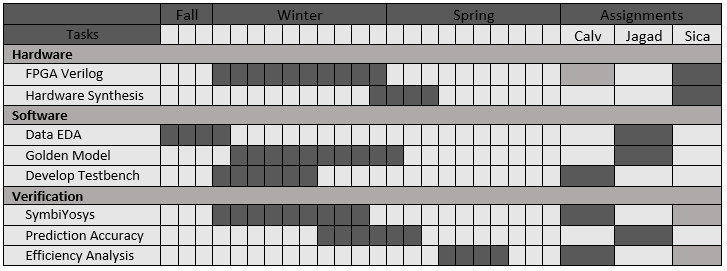
\includegraphics[width=\linewidth]{gantt.png}
\end{table}
%\section{Programming Source Code and Drawings}
\end{appendices}
\end{document}

%\begin{figure}[!htb]
%  \centering
%  \includegraphics[width=4in]{}
%  \caption{}\label{fig:}
%\end{figure}

%%% Local Variables:
%%% mode: latex
%%% TeX-master: t
%%% End:
